%!TEX TS-program = pdflatex
%!TEX root = tesi.tex
%!TEX encoding = UTF-8 Unicode


\section{Primo Assignment}

%TODO poche parole di recap


\subsection{System Concept Statement}

Ricettavola, ricette da favola da mettere in tavola, permette di raccogliere e condividere ricette da cucina.
Pensata per studenti e lavoratori, fornisce, a partire dalle ricette selezionate, la possibilità di generare liste della spesa in velocità;
in questo modo anche l'utente più distratto non si dimenticherà nessun ingrediente.
In modalità "Assistente" verranno mostrati uno ad uno ed in ordine i passaggi per la preparazione della ricetta selezionata.
Condividere, esportare ed importare ricette con amici e colleghi sarà facile e veloce.
Le ricette potranno essere modificate in modo da essere adattate ad ogni palato.
I più fantasiosi potranno creare nuove ricette specificando ingredienti, passaggi, e tempo necessari alla preparazione.
Le ricette saranno identificate dal loro nome e da una foto.
Ricettavola fornisce un unico strumento per raccolta e la preparazione di ricette per ottimi pranzi e cene.







\subsection{Storyboarding}
\subsubsection{Primo Storyboard}

In figura~\ref{fig:storyboard_1} è illustrata una prima versione dello storyboard.
Segue una breve descrizione di ciascun pannello.
\begin{enumerate}
  \item Le scene iniziali avranno luogo in un'università.
  \item Mario racconta preoccupato ad un suo amico che Marta verrà a cena a casa sua.
  \item Mario è impreparato e non sa cosa cucinare.
    Allora l'amico gli consiglia una sua ricetta e gliela invia con Ricettavola.
    Mario non si tranquillizza perché sa di avere il frigorifero vuoto.
  \item L'amico spiega che c'è un modo per creare liste della spesa.
  \item La scena si sposta all'esterno di un supermercato, si capisce che Mario ha comprato tutto il necessario.
  \item Tornato a casa Mario avvia la modalità "Assistente" di Ricettavola.
  \item Mario segue i passaggi della ricetta.
  \item Nell'ultimo pannello si vede che Mario è riuscito a cucinare un'ottima cena.
\end{enumerate}

\clearpage
\begin{figure}[!ht]
  \begin{center}
    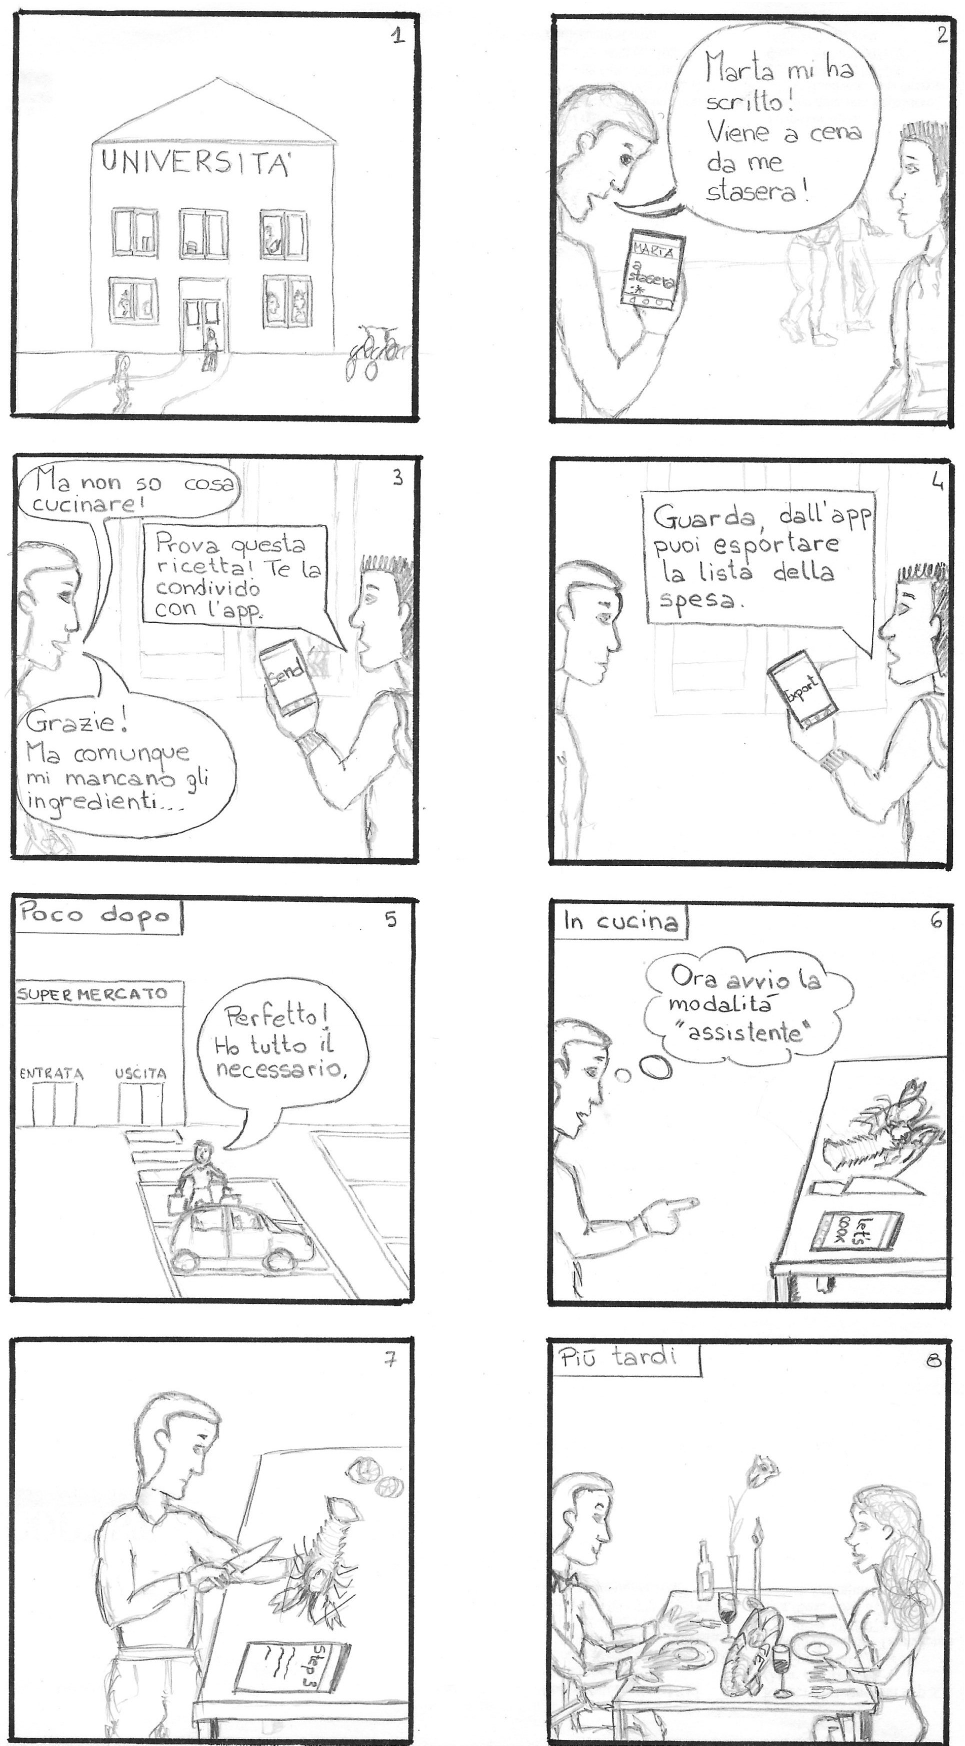
\includegraphics[height=0.9\textheight,keepaspectratio]{storyboard_1}
    \caption{Primo storyboard}
    \label{fig:storyboard_1}
  \end{center}
\end{figure}
\clearpage

Dopo aver testato la chiarezza dello storyboard sono emerse alcune problematiche:
\begin{itemize}
  \item la maggior parte degli intervistati ha creduto che l'applicazione fornisse un elenco di ricette online;

  \item non viene illustrata la creazione di una ricetta;

  \item il nome dell'applicazione non viene mai menzionato;

  \item non si capisce che la ricetta è stata creata dall'amico;

  \item la parola "esporta" fa pensare a funzionalità esterne all'applicazione, gli intervistati pensano che venga richiesta un'altra applicazione per la gestione della lista della spesa;
\end{itemize}

\subsubsection{Storyboard Finale}

Nello storyboard in figura~\ref{fig:storyboard_2} l'attenzione si concentra sui passaggi di creazione, preparazione e condivisione di una ricetta.
%Si è preferito omettere l'informazione riguardo la lista della spesa perché ritenuta accessoria rispetto alle funzionalità principali di Ricettavola.

Segue una breve descrizione di ciascun pannello.
\begin{enumerate}
  \item Luca chiede a sua nonna se può salvare su Ricettavola la sua ricetta per la torta alle pere.
  \item Dal pannello si capisce che Luca ha creato una nuova ricetta ed ha salvato tutti i dettagli.
  \item Luca, giunto a casa, inizia a cucinare supportato dalla modalità "Assistente" di Ricettavola.
  \item Luca è riuscito a preparare un'ottima torta e consiglia l'applicazione ad una sua amica.
  \item Dal pannello si capisce che Luca ha appena condiviso la ricetta della torta alle pere.
\end{enumerate}

\clearpage
\begin{figure}[!ht]
  \begin{center}
    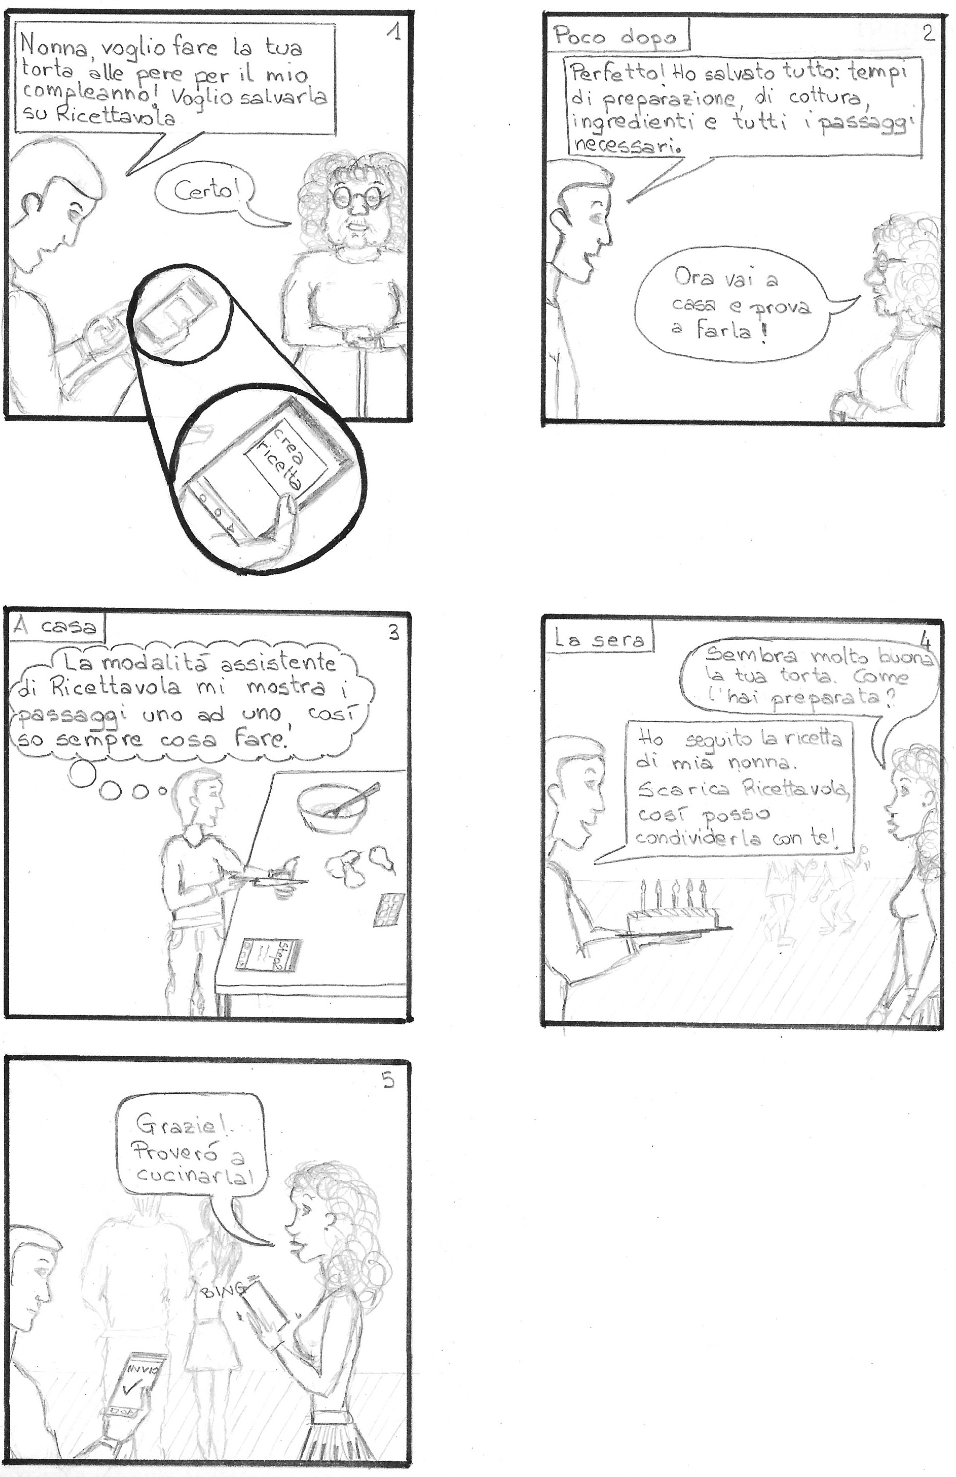
\includegraphics[height=0.9\textheight,keepaspectratio]{storyboard_2}
    \caption{Storyboard Finale}
    \label{fig:storyboard_2}
  \end{center}
\end{figure}
\clearpage

Lo storyboard in figura~\ref{fig:storyboard_2} è risultato molto più chiaro, infatti tutti gli intervistati hanno compreso ogni pannello e i passaggi tra i vari pannelli.
Ora sono consapevoli di dover raccogliere le ricette in maniera attiva, creandole oppure ricevendole da amici.


\subsection{Requirements Brief}
TODO
TODOOOOOOOOOOOOOOOOO
\subsubsection{What}
\subsubsection{Why}
\subsubsection{Goal and Audience}

%\subsection{Personas}
% Se avanza tempo
